% -- --------------------------------------------------------------------------------------------------- -- %
% -- Proyecto:                                                                                           -- %
% -- Archivo: reporte.rnw                                                                                -- %
% -- Repositorio: https://github.com/IFFranciscoME/A1_Temporal_Patterns                                  -- %
% -- Autor: Francisco ME                                                                                 -- %
% -- --------------------------------------------------------------------------------------------------- -- %

\documentclass{iteraposter}\usepackage[]{graphicx}\usepackage[]{color}
% maxwidth is the original width if it is less than linewidth
% otherwise use linewidth (to make sure the graphics do not exceed the margin)
\makeatletter
\def\maxwidth{ %
  \ifdim\Gin@nat@width>\linewidth
    \linewidth
  \else
    \Gin@nat@width
  \fi
}
\makeatother

\definecolor{fgcolor}{rgb}{0.345, 0.345, 0.345}
\newcommand{\hlnum}[1]{\textcolor[rgb]{0.686,0.059,0.569}{#1}}%
\newcommand{\hlstr}[1]{\textcolor[rgb]{0.192,0.494,0.8}{#1}}%
\newcommand{\hlcom}[1]{\textcolor[rgb]{0.678,0.584,0.686}{\textit{#1}}}%
\newcommand{\hlopt}[1]{\textcolor[rgb]{0,0,0}{#1}}%
\newcommand{\hlstd}[1]{\textcolor[rgb]{0.345,0.345,0.345}{#1}}%
\newcommand{\hlkwa}[1]{\textcolor[rgb]{0.161,0.373,0.58}{\textbf{#1}}}%
\newcommand{\hlkwb}[1]{\textcolor[rgb]{0.69,0.353,0.396}{#1}}%
\newcommand{\hlkwc}[1]{\textcolor[rgb]{0.333,0.667,0.333}{#1}}%
\newcommand{\hlkwd}[1]{\textcolor[rgb]{0.737,0.353,0.396}{\textbf{#1}}}%
\let\hlipl\hlkwb

\usepackage{framed}
\makeatletter
\newenvironment{kframe}{%
 \def\at@end@of@kframe{}%
 \ifinner\ifhmode%
  \def\at@end@of@kframe{\end{minipage}}%
  \begin{minipage}{\columnwidth}%
 \fi\fi%
 \def\FrameCommand##1{\hskip\@totalleftmargin \hskip-\fboxsep
 \colorbox{shadecolor}{##1}\hskip-\fboxsep
     % There is no \\@totalrightmargin, so:
     \hskip-\linewidth \hskip-\@totalleftmargin \hskip\columnwidth}%
 \MakeFramed {\advance\hsize-\width
   \@totalleftmargin\z@ \linewidth\hsize
   \@setminipage}}%
 {\par\unskip\endMakeFramed%
 \at@end@of@kframe}
\makeatother

\definecolor{shadecolor}{rgb}{.97, .97, .97}
\definecolor{messagecolor}{rgb}{0, 0, 0}
\definecolor{warningcolor}{rgb}{1, 0, 1}
\definecolor{errorcolor}{rgb}{1, 0, 0}
\newenvironment{knitrout}{}{} % an empty environment to be redefined in TeX

\usepackage{alltt}

\usepackage{lipsum}                                % Dummy text
\usepackage[absolute, overlay]{textpos}            % Figure placement
\setlength{\TPHorizModule}{\paperwidth}
\setlength{\TPVertModule}{\paperheight}


\title{
  Clustering subsecuencial de series de tiempo: Evidencia de patrones temporales en el
  tipo de cambio USD/MXN
  }

\vskip4cm

\author {
  Juan Francisco Mu\~noz Elguez\'abal \inst{1}
  \and
  Riemann Ru\'iz Cruz \inst{2}
  }

\institute {
  \inst{1} Msc. Ciencia de Datos - ITESO
  \and
  \inst{2} Departamento de Matem\'aticas y F\'isca - ITESO
  }

% -- --------------------------------------------------------------------------- Comienzo de codigo en R -- %

% -- Reunion con Diana y Juan Diego para hablar del proceso de generacion del regresor.









\IfFileExists{upquote.sty}{\usepackage{upquote}}{}
\begin{document}

\begin{frame}

% -- -------------------------------------------------------------------------------------- 1er Renglon -- %
% -- -------------------------------------------------------------------------------------- ----------- -- %

\begin{columns}[onlytextwidth]
  
  \begin{column}{.75 \textwidth - 0.01 \textwidth}
    \begin{block}{Hip\'otesis - Experimento}
    
    \textbf{Hip\'otesis: } \\
      Existe un conjunto de condiciones bajo las cuales, la ocurrencia de evento ex\'ogeno a una serie de
      tiempo financiera, provoca la presencia de patrones temporales observables en la misma serie.
      
    \textbf{Experimento: } \\
      Comunicado de indicadores macroecon\'omicos de M\'exico y USA, como candidatos de eventos generadores
      de patrones temporales en la serie de tiempo intrad\'ia del del tipo de cambio USD/MXN.
      
    \end{block}
  \end{column}


\begin{column}{.25 \textwidth - 0.01 \textwidth}
  \begin{block}{Informacion general}
        
    \begin{itemize}
      \item 10 a\~nos de informaci\'on.
      \item 2010-01-01 al 2020-01-03
      \item 14.5 Millones de precios.
      \item 36,000 comunicados de indicadores.
      \item indicadores econ\'omicos de \textit{factset}.
      \item precios del broker regulado \textit{Oanda}.
    \end{itemize}
      
  \end{block}
\end{column}
\end{columns}

% -- -------------------------------------------------------------------------------------- 2do Renglon -- %
% -- -------------------------------------------------------------------------------------- ----------- -- %

\begin{columns}[onlytextwidth]
  
  \begin{column}{.5 \textwidth - 0.01 \textwidth}
    \begin{block}{Definiciones}
    
      Sea el proceso $\left\{ S_{T} \right\}_{T=1}^{n}$,
      como los precios $OHLC_{T}: \left\{ Open_{T}, High_{T}, Low_{T}, Close_{T} \right\}$ de cada $n$
      minuto $burs\'atil$ de los \'ultimos 10 a\~nos.
      De los cuales se extraen ventanas de tama\~no $m$, de tal manera que
      $\left\{ OHLC_{t} \right\}_{t=1}^{m} $, para $m = 30$.

      \begin{itemize}
        \item \textbf{micro-volatilidades:} $\rightarrow$ $HL_{t} = High_{t} - Low_{t}$
        \item \textbf{micro-rendimientos:} $\rightarrow$ $OC_{t} = Open_{t} - Close_{t}$
      \end{itemize}
      
      Sea el proceso $\left\{ I_{t} \right\}_{t=1}^{k}$ como el comunicado de un indicador macroecon\'omico
      que sucede $k$ veces, tal que, con $OHLC_{k}
      \left\{ Open_{t=1:m}^{k}, High_{t=1:m}^{k}, Low_{t=1:m}^{k}, Close_{t=1:m}^{k} \right\}$
      se definen las series de tiempo $OC_{t=1:m}^{k}$ y $HL_{1:m}^{k}$ como \textit{motifs} para encontrar en
      $OHLC_{T}$

    \end{block}
  \end{column}

  \begin{column}{.5 \textwidth - 0.01\textwidth}
    \begin{block}{Ej: Ventana $k=1$ de $m=30$ Precios OHLC}
      \begin{figure}[H]
        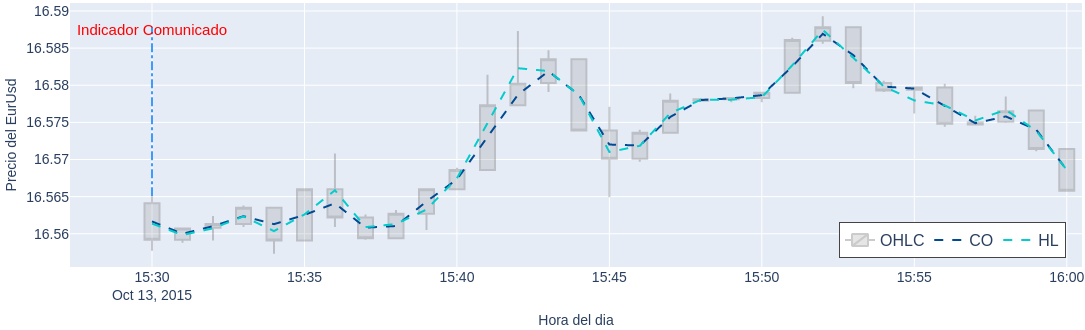
\includegraphics[scale=1]{imagenes/grafica_1.png}
      \end{figure}
    \end{block}
  \end{column}
  
\end{columns}



% -- -------------------------------------------------------------------------------------- 3er Renglon -- %
% -- -------------------------------------------------------------------------------------- ----------- -- %

\begin{columns}[onlytextwidth]
  
  \begin{column}{.25 \textwidth - 0.01 \textwidth}
    \begin{block}{Categor\'ias}
      \centering
      \small
      
\begin{tabular}{c|c|c|c}
\hline
categoria & usa & mex & total\\
\hline
actividad economica & 26 & 7 & 33\\
\hline
consumo & 29 & 5 & 34\\
\hline
energia & 4 & 0 & 4\\
\hline
flujos de capital & 5 & 0 & 5\\
\hline
inflacion & 0 & 4 & 4\\
\hline
mercado inmobiliario & 11 & 1 & 12\\
\hline
mercado laboral & 13 & 2 & 15\\
\hline
subasta de bonos & 5 & 0 & 5\\
\hline
tasas de interes & 1 & 1 & 2\\
\hline
total & 94 & 20 & 114\\
\hline
\end{tabular}


      \normalsize
    \end{block}
  \end{column}

  \begin{column}{.5 \textwidth - 0.01 \textwidth}
    \begin{block}{Indicadores}
      Grafica 
    \end{block}
  \end{column}
  
  \begin{column}{.25 \textwidth - 0.01 \textwidth}
    \begin{block}{Indicadores}
      Preguntas
    \end{block}
  \end{column}

\end{columns}

% -- -------------------------------------------------------------------------------------- 4to Renglon -- %
% -- -------------------------------------------------------------------------------------- ----------- -- %

\begin{columns}[onlytextwidth]
  
  \begin{column}{.33 \textwidth - 0.01 \textwidth}
    \begin{block}{Similitud entre series de tiempo}
      \begin{equation}
        \hat{x} = \frac{x_{i}-\mu_{x}}{\sigma_{x}} , \hat{y} = \frac{y_{i}-\mu_{y}}{\sigma_{y}}
      \end{equation}
      \begin{equation}
        d(x,y) = \sqrt{\sum_{i=1}^{n}(\hat{x_{i}} -\hat{y_{i}})^{2})}
      \end{equation}
      \end{block}
  \end{column}

  \begin{column}{.33 \textwidth - 0.01 \textwidth}
    \begin{block}{Algoritmo MASS}
      Algoritmo
    \end{block}
  \end{column}
  
  \begin{column}{.33 \textwidth - 0.01 \textwidth}
    \begin{block}{Complejidad}
      algoritmo
    \end{block}
  \end{column}

\end{columns}

% -- -------------------------------------------------------------------------------------- 4to Renglon -- %
% -- -------------------------------------------------------------------------------------- ----------- -- %

\begin{columns}[onlytextwidth]
  
  \begin{column}{.25 \textwidth - 0.01 \textwidth}
    \begin{block}{Resultados 1}
      \begin{figure}[H]
        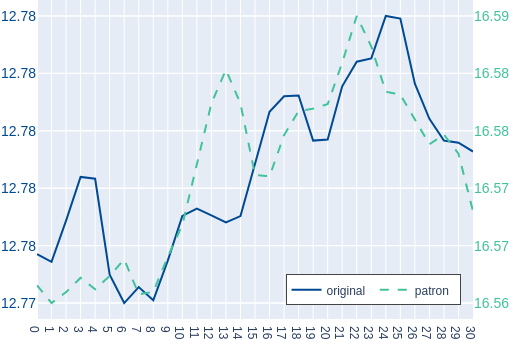
\includegraphics[scale=1]{imagenes/grafica_2.png}
      \end{figure}
      \end{block}
  \end{column}

  \begin{column}{.25 \textwidth - 0.01 \textwidth}
    \begin{block}{Resultados 3}
      
    \end{block}
  \end{column}
  
  \begin{column}{.50 \textwidth - 0.01 \textwidth}
    \begin{block}{Resultados 3}
      \begin{figure}[H]
        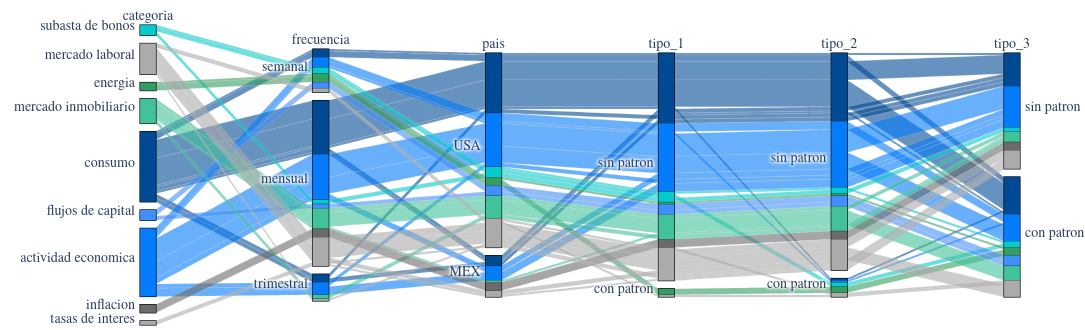
\includegraphics[scale=1]{imagenes/grafica_3.png}
      \end{figure}
    \end{block}
  \end{column}
  
\end{columns}

\end{frame}
\end{document}
